\documentclass[11pt,a4paper]{article}

% --- Packages ---
\usepackage[utf8]{inputenc}
\usepackage[margin=1in]{geometry}
\usepackage{amsmath,amssymb}
\usepackage{graphicx}
\usepackage{booktabs}
\usepackage{listings}
\usepackage{xcolor}
\usepackage{fancyhdr}
\usepackage{microtype}
\usepackage{tikz}
\usepackage{enumitem}
\usepackage{pifont}
\usepackage{mdframed}
\usetikzlibrary{arrows.meta, positioning, shapes.geometric, calc, shapes.multipart}

% --- Hyperref Setup ---
\usepackage{hyperref}
\hypersetup{
    colorlinks=true,
    linkcolor=blue,
    citecolor=red,
    urlcolor=teal,
    pdftitle={WebRTC Phase 1 - Issue \#1: Backend Setup \& API},
    pdfauthor={WebRTC Engineering Team}
}
\usepackage{cleveref}

% --- Custom Page Layout ---
\pagestyle{fancy}
\fancyhf{}
\setlength{\headheight}{14.5pt}
\rhead{\textbf{WebRTC Phase 1 --- Issue \#1}}
\lhead{Backend Setup \& API Documentation}
\rfoot{Page \thepage}
\lfoot{Confidential --- For Internal Use Only}
\renewcommand{\headrulewidth}{0.4pt}
\renewcommand{\footrulewidth}{0.4pt}

% --- Color Definitions ---
\definecolor{codegray}{rgb}{0.96,0.96,0.96}
\definecolor{codeblue}{rgb}{0.1,0.2,0.6}
\definecolor{codegreen}{rgb}{0.1,0.5,0.1}
\definecolor{codeorange}{rgb}{0.8,0.4,0.0}
\definecolor{successgreen}{rgb}{0.0,0.55,0.27}
\definecolor{warningred}{rgb}{0.75,0.1,0.1}
\definecolor{infobox}{rgb}{0.9,0.95,1.0}
\definecolor{borderblue}{rgb}{0.2,0.4,0.8}

% --- Code Block Style ---
\lstset{
    backgroundcolor=\color{codegray},
    basicstyle=\small\ttfamily,
    breakatwhitespace=false,
    breaklines=true,
    captionpos=b,
    commentstyle=\color{codegreen},
    keywordstyle=\color{codeblue}\bfseries,
    stringstyle=\color{codeorange},
    numbers=left,
    numberstyle=\tiny\color{gray},
    numbersep=5pt,
    showspaces=false,
    showstringspaces=false,
    showtabs=false,
    tabsize=2,
    frame=single,
    rulecolor=\color{lightgray}
}

\lstdefinelanguage{json}{
    stringstyle=\color{codeblue},
    string=[s]{"}{"},
    comment=[l]{//},
    morecomment=[s]{/*}{*/},
    morestring=[b]',
}

\lstdefinelanguage{bash}{
    morekeywords={npm, node, curl, mkdir, cd, git},
    keywordstyle=\color{codeblue}\bfseries,
    commentstyle=\color{codegreen},
    comment=[l]{\#},
    basicstyle=\small\ttfamily,
}

% --- Custom Status Box ---
\newmdenv[
    backgroundcolor=infobox,
    linecolor=borderblue,
    linewidth=1.5pt,
    roundcorner=5pt,
    innertopmargin=6pt,
    innerbottommargin=6pt,
    innerleftmargin=10pt,
    innerrightmargin=10pt
]{infoblock}

% --- Document Info ---
\title{
    \vspace{1.5in}
    \Huge \textbf{WebRTC One-to-One Video Call} \\
    \Large Phase 1 --- Backend \& Signaling Foundation \\
    \vspace{0.5in}
    \huge \textbf{Issue \#1: Backend Setup \& API} \\
    \large \textit{Day 1 Sprint Documentation} \\
    \vspace{1.5in}
}
\author{
    \textbf{Assignee:} Aabhishek23 \\[0.3em]
    \textbf{Repository:} Aabhishek23/WEBRTC \\[0.3em]
    \textbf{Labels:} \texttt{enhancement · backend · setup · api · Day-1}
}
\date{June 29, 2026}

\begin{document}

\maketitle
\thispagestyle{empty}
\newpage

\tableofcontents
\newpage

% =========================================================================
\section{Issue Overview}
% =========================================================================

\begin{infoblock}
\textbf{Issue ID:} \texttt{ISSUE-001} \quad
\textbf{Day:} 1 \quad
\textbf{Type:} Feature \quad
\textbf{Priority:} High \quad
\textbf{Status:} \textcolor{successgreen}{\textbf{Completed}} \\[0.4em]
\textbf{Estimated Hours:} 4 hrs \quad
\textbf{Milestone:} M1 --- Server Foundation (Day 1--2)
\end{infoblock}

\vspace{0.5em}

\subsection{Objective}

This issue covers the complete setup of the \textbf{Node.js + Express.js} backend server for the WebRTC One-to-One Video Call application (Phase 1). The goal is to establish a working HTTP server with:

\begin{itemize}
    \item Proper environment configuration via \texttt{dotenv}
    \item A \textbf{room creation API} (\texttt{POST /api/rooms}) returning a unique \texttt{XXX-XXX-XXX} room ID
    \item A \textbf{health check} endpoint (\texttt{GET /api/health})
    \item Modular folder structure for scalability in Phase 2
\end{itemize}

\subsection{Scope}

\begin{table}[h!]
\centering
\begin{tabular}{@{}lll@{}}
\toprule
\textbf{Component} & \textbf{Technology} & \textbf{Purpose} \\ \midrule
HTTP Server         & Node.js + Express.js   & API request handling \\
Environment Config  & dotenv                 & Secure config management \\
Room ID Generator   & Custom utility         & Unique XXX-XXX-XXX format IDs \\
Error Handling      & Express middleware      & Structured JSON error responses \\
Dev Server          & nodemon                & Auto-restart on file change \\ \bottomrule
\end{tabular}
\caption{Technology Stack for Issue \#1}
\label{tab:tech_stack}
\end{table}

% =========================================================================
\section{Project Structure}
% =========================================================================

\subsection{Directory Layout}

The backend code resides inside the \texttt{server/} folder at the root of the repository. The folder structure implemented during this issue is:

\begin{lstlisting}[language=bash, caption={Backend Folder Structure}, label={lst:folder}]
WEBRTC/
  server/
    middleware/
      errorHandler.js       # Global error handling middleware
    routes/
      rooms.js              # POST /api/rooms + GET /api/rooms/:id
    utils/
      roomIdGenerator.js    # XXX-XXX-XXX room ID generator
    .env                    # Local environment variables (git-ignored)
    .env.example            # Template for environment setup
    package.json            # Project metadata & scripts
    server.js               # Main Express server entry point
\end{lstlisting}

\subsection{Design Rationale}

The folder structure follows the \textbf{Separation of Concerns} principle:

\begin{itemize}
    \item \textbf{Routes} contain only HTTP handler logic --- no business logic.
    \item \textbf{Utils} hold reusable pure functions (e.g., ID generation).
    \item \textbf{Middleware} captures cross-cutting concerns (errors, logging).
    \item \textbf{server.js} is the composition root --- it wires everything together.
\end{itemize}

This structure is forward-compatible with \textbf{Day 2 (Socket.IO)} and \textbf{Day 3 (Signaling)} additions without requiring refactoring.

% =========================================================================
\section{API Specification}
% =========================================================================

\subsection{POST /api/rooms}

Creates a new room and returns a unique 9-digit room ID.

\begin{table}[h!]
\centering
\begin{tabular}{@{}ll@{}}
\toprule
\textbf{Field}          & \textbf{Value} \\ \midrule
Method                  & \texttt{POST} \\
Endpoint                & \texttt{/api/rooms} \\
Authentication          & None (Phase 1) \\
Request Body            & Empty \\
Content-Type            & \texttt{application/json} \\
Success Status Code     & \texttt{201 Created} \\ \bottomrule
\end{tabular}
\caption{POST /api/rooms Endpoint Specification}
\label{tab:post_rooms}
\end{table}

\subsubsection{Success Response}

\begin{lstlisting}[language=json, caption={POST /api/rooms --- 201 Created Response}]
{
  "success": true,
  "roomId": "346-661-586",
  "message": "Room created successfully",
  "createdAt": "2026-06-28T18:30:03.418Z"
}
\end{lstlisting}

\subsubsection{Error Response}

\begin{lstlisting}[language=json, caption={POST /api/rooms --- 500 Internal Server Error}]
{
  "success": false,
  "message": "Internal Server Error",
  "stack": "Error: ... (only in development mode)"
}
\end{lstlisting}

% ---

\subsection{GET /api/health}

Server liveness check --- returns current environment and timestamp.

\begin{table}[h!]
\centering
\begin{tabular}{@{}ll@{}}
\toprule
\textbf{Field}      & \textbf{Value} \\ \midrule
Method              & \texttt{GET} \\
Endpoint            & \texttt{/api/health} \\
Success Status Code & \texttt{200 OK} \\ \bottomrule
\end{tabular}
\caption{GET /api/health Endpoint Specification}
\label{tab:get_health}
\end{table}

\subsubsection{Success Response}

\begin{lstlisting}[language=json, caption={GET /api/health --- 200 OK Response}]
{
  "status": "OK",
  "environment": "development",
  "timestamp": "2026-06-28T18:29:24.094Z"
}
\end{lstlisting}

% ---

\subsection{GET /api/rooms/:roomId}

Checks whether a given room ID is currently active.

\begin{lstlisting}[language=json, caption={GET /api/rooms/346-661-586 --- 200 OK}]
{
  "success": true,
  "roomId": "346-661-586",
  "message": "Room exists"
}
\end{lstlisting}

\begin{lstlisting}[language=json, caption={GET /api/rooms/000-000-000 --- 404 Not Found}]
{
  "success": false,
  "message": "Room 000-000-000 not found"
}
\end{lstlisting}

\newpage

% =========================================================================
\section{Implementation Details}
% =========================================================================

\subsection{Room ID Generation Algorithm}

The unique room ID generator is the core business logic of this issue. The algorithm uses an \textbf{in-memory \texttt{Set}} to guarantee no duplicate IDs are issued during the server's lifetime.

\begin{lstlisting}[language=java, caption={roomIdGenerator.js --- Core Algorithm}]
const activeRooms = new Set();

const generateRoomId = () => {
  let roomId;
  do {
    // Generate 9 random digits
    const digits = Math.floor(
      100000000 + Math.random() * 900000000
    ).toString();
    // Format as XXX-XXX-XXX
    roomId = `${digits.slice(0,3)}-${digits.slice(3,6)}-${digits.slice(6,9)}`;
  } while (activeRooms.has(roomId)); // Retry if duplicate

  activeRooms.add(roomId);
  return roomId;
};
\end{lstlisting}

\subsubsection{Algorithm Properties}

\begin{itemize}
    \item \textbf{Format:} \texttt{XXX-XXX-XXX} where each \texttt{X} is a digit (0--9)
    \item \textbf{Search Space:} $9 \times 10^8 = 900{,}000{,}000$ possible room IDs
    \item \textbf{Collision Probability (first call):} $\approx 0$ (practically zero for Phase 1 scale)
    \item \textbf{Duplicate Prevention:} \texttt{do-while} loop with \texttt{Set.has()} check
    \item \textbf{Time Complexity:} $O(1)$ average case
\end{itemize}

\subsection{Server Entry Point}

The \texttt{server.js} file is the application's composition root. It:

\begin{enumerate}
    \item Loads environment variables via \texttt{dotenv.config()}
    \item Attaches JSON body parser middleware
    \item Registers the \texttt{/api/rooms} route
    \item Registers the \texttt{/api/health} inline route
    \item Attaches the global error handler as the last middleware
    \item Starts listening on the configured \texttt{PORT}
\end{enumerate}

\begin{lstlisting}[language=java, caption={server.js -- Middleware Pipeline}]
dotenv.config();
app.use(express.json());          // Parse JSON bodies
app.use('/api/rooms', roomRoutes); // Room management routes
app.get('/api/health', handler);   // Health check
app.use(errorHandler);             // Must be LAST middleware
app.listen(PORT, callback);
\end{lstlisting}

\begin{infoblock}
\textbf{Important:} The \texttt{errorHandler} middleware \textbf{must} be registered after all routes. Express identifies error-handling middleware by its 4-parameter signature: \texttt{(err, req, res, next)}.
\end{infoblock}

\subsection{Environment Configuration}

\begin{lstlisting}[language=bash, caption={.env.example --- Environment Template}]
# Server Environment Configuration
# Copy this file to .env and fill in your values

PORT=5000
NODE_ENV=development
\end{lstlisting}

\begin{itemize}
    \item \texttt{.env} is listed in \texttt{.gitignore} to prevent accidental credential commits.
    \item \texttt{.env.example} is committed as a reference template for new developers.
    \item \texttt{process.env.PORT || 5000} fallback ensures the server works even without \texttt{.env}.
\end{itemize}

\newpage

% =========================================================================
\section{Request--Response Flow Diagram}
% =========================================================================

\begin{figure}[h!]
\centering
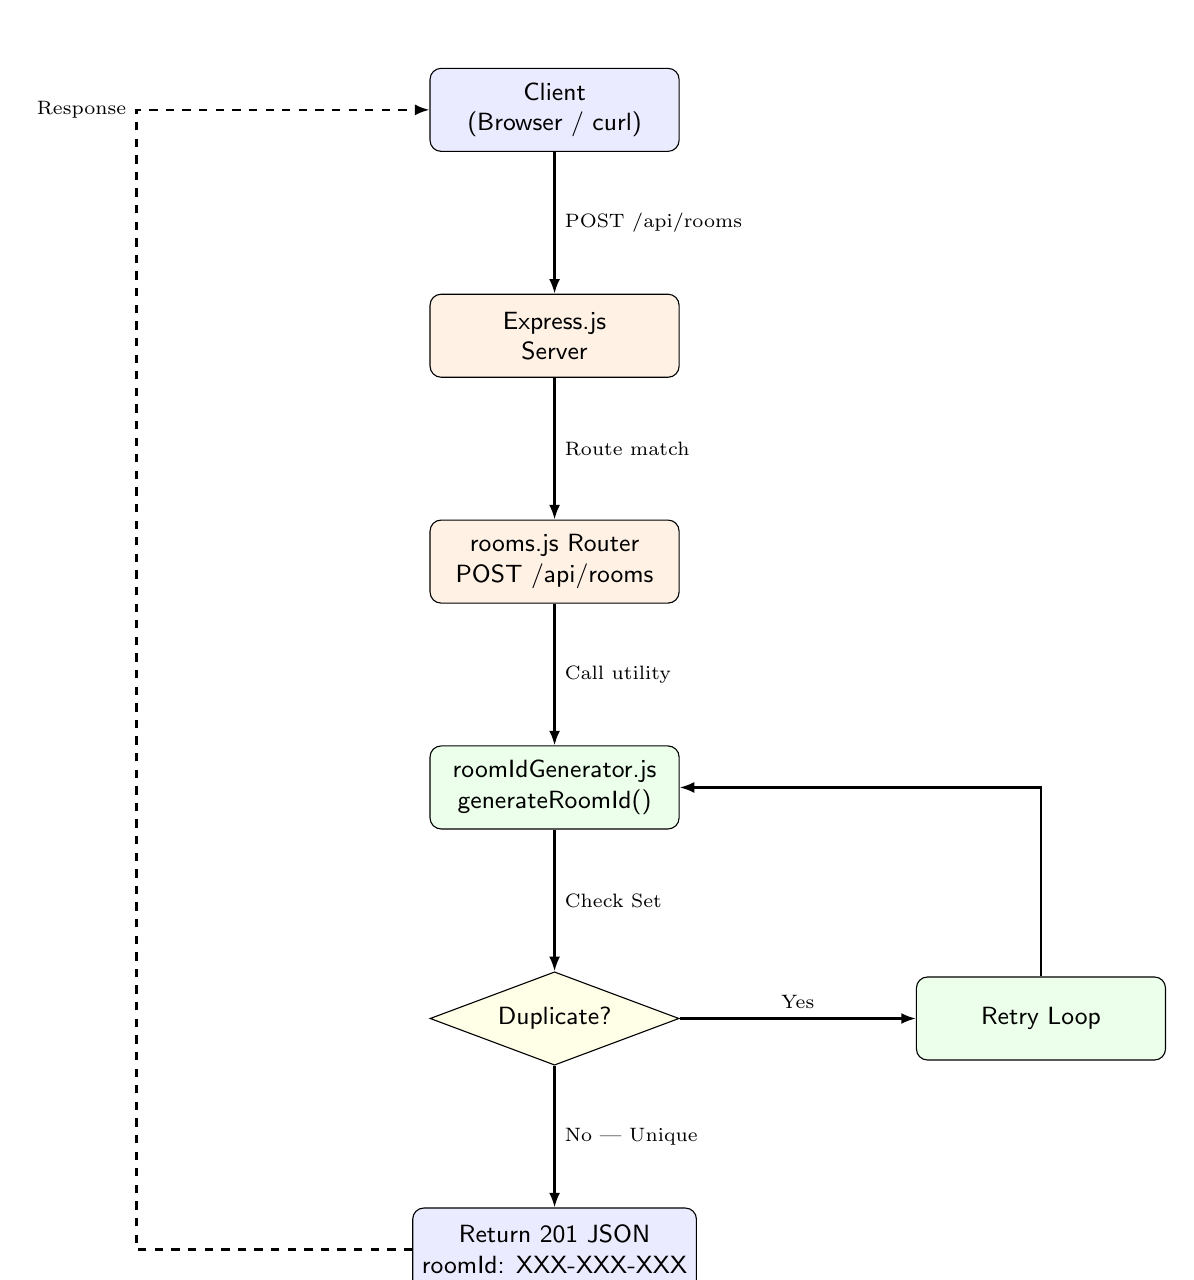
\begin{tikzpicture}[
    node distance=1.8cm and 3.5cm,
    box/.style={draw, fill=blue!8, rectangle, minimum height=3em,
                minimum width=9em, rounded corners, align=center,
                font=\small\sffamily},
    middleware/.style={draw, fill=orange!10, rectangle, minimum height=3em,
                       minimum width=9em, rounded corners, align=center,
                       font=\small\sffamily},
    util/.style={draw, fill=green!8, rectangle, minimum height=3em,
                 minimum width=9em, rounded corners, align=center,
                 font=\small\sffamily},
    decision/.style={draw, fill=yellow!10, diamond, aspect=2.5,
                     minimum width=9em, align=center, font=\small\sffamily},
    line/.style={draw, -{Latex[scale=0.8]}, thick}
]

    \node[box]        (client)    {Client\\(Browser / curl)};
    \node[middleware, below=of client]  (express)   {Express.js\\Server};
    \node[middleware, below=of express] (router)    {rooms.js Router\\POST /api/rooms};
    \node[util, below=of router]        (generator) {roomIdGenerator.js\\generateRoomId()};
    \node[decision, below=of generator] (check)     {Duplicate?};
    \node[util, right=3cm of check]     (retry)     {Retry Loop};
    \node[box, below=of check]          (respond)   {Return 201 JSON\\roomId: XXX-XXX-XXX};

    \draw[line] (client)    -- node[right, font=\scriptsize]{POST /api/rooms} (express);
    \draw[line] (express)   -- node[right, font=\scriptsize]{Route match} (router);
    \draw[line] (router)    -- node[right, font=\scriptsize]{Call utility} (generator);
    \draw[line] (generator) -- node[right, font=\scriptsize]{Check Set} (check);
    \draw[line] (check.east) -- node[above, font=\scriptsize]{Yes} (retry.west);
    \draw[line] (retry.north) |- (generator.east);
    \draw[line] (check)     -- node[right, font=\scriptsize]{No --- Unique} (respond);
    \draw[line, dashed] (respond.west) -- ++(-3.5,0) |- (client.west)
        node[midway, left, font=\scriptsize]{Response};

\end{tikzpicture}
\caption{POST /api/rooms --- Complete Request--Response Flow}
\label{fig:request_flow}
\end{figure}

% =========================================================================
\section{Testing \& Verification}
% =========================================================================

\subsection{Manual Test Results}

All acceptance criteria were verified using \texttt{curl} against the running server at \texttt{http://localhost:5000}.

\subsubsection{Test 1 --- Health Check Endpoint}

\begin{lstlisting}[language=bash, caption={Health Check curl Command}]
curl -s http://localhost:5000/api/health
\end{lstlisting}

\begin{lstlisting}[language=json, caption={Health Check --- Actual Output}]
{
  "status": "OK",
  "environment": "development",
  "timestamp": "2026-06-28T18:29:24.094Z"
}
\end{lstlisting}

\textbf{Result:} \textcolor{successgreen}{\textbf{PASS}} \ding{51}

\vspace{0.8em}

\subsubsection{Test 2 --- Room Creation}

\begin{lstlisting}[language=bash, caption={Room Creation curl Command}]
curl -s -X POST http://localhost:5000/api/rooms \
     -H "Content-Type: application/json"
\end{lstlisting}

\begin{lstlisting}[language=json, caption={Room Creation --- Actual Output}]
{
  "success": true,
  "roomId": "346-661-586",
  "message": "Room created successfully",
  "createdAt": "2026-06-28T18:30:03.418Z"
}
\end{lstlisting}

\textbf{Result:} \textcolor{successgreen}{\textbf{PASS}} \ding{51} --- Room ID format \texttt{346-661-586} matches \texttt{XXX-XXX-XXX}

\subsection{Acceptance Criteria Verification}

\begin{table}[h!]
\centering
\begin{tabular}{@{}lcc@{}}
\toprule
\textbf{Acceptance Criterion} & \textbf{Expected} & \textbf{Status} \\ \midrule
Server starts on configured PORT                     & PORT 5000         & \textcolor{successgreen}{\textbf{PASS}} \\
POST /api/rooms returns XXX-XXX-XXX format ID        & 346-661-586       & \textcolor{successgreen}{\textbf{PASS}} \\
Environment variables load from \texttt{.env}        & NODE\_ENV=dev     & \textcolor{successgreen}{\textbf{PASS}} \\
Duplicate room IDs not generated                     & Set prevents dup  & \textcolor{successgreen}{\textbf{PASS}} \\
GET /api/health returns 200 OK                       & status: OK        & \textcolor{successgreen}{\textbf{PASS}} \\ \bottomrule
\end{tabular}
\caption{Acceptance Criteria Verification Results}
\label{tab:acceptance}
\end{table}

\vspace{1em}
\begin{infoblock}
\textbf{All 5 acceptance criteria verified and passed.}\\
Issue \#1 is complete and ready for merge into \texttt{main}.
\end{infoblock}

\newpage

% =========================================================================
\section{npm Scripts Reference}
% =========================================================================

\begin{table}[h!]
\centering
\begin{tabular}{@{}lll@{}}
\toprule
\textbf{Script} & \textbf{Command} & \textbf{Use Case} \\ \midrule
\texttt{npm run dev}   & \texttt{nodemon server.js} & Development (auto-restart) \\
\texttt{npm start}     & \texttt{node server.js}    & Production server start \\
\texttt{npm test}      & Echo placeholder           & Placeholder (Day 7 tests) \\ \bottomrule
\end{tabular}
\caption{Available npm Scripts}
\label{tab:npm_scripts}
\end{table}

\subsection{Installing Dependencies}

\begin{lstlisting}[language=bash, caption={Dependency Installation}]
# Navigate to server folder
cd server/

# Install production dependencies
npm install express dotenv uuid

# Install development dependency
npm install --save-dev nodemon
\end{lstlisting}

\subsection{Installed Packages}

\begin{table}[h!]
\centering
\begin{tabular}{@{}llll@{}}
\toprule
\textbf{Package} & \textbf{Version} & \textbf{Type} & \textbf{Purpose} \\ \midrule
express  & \textasciicircum 4.x & Production    & HTTP server framework \\
dotenv   & \textasciicircum 16.x & Production   & Environment variable loader \\
uuid     & \textasciicircum 9.x  & Production   & Available for future use \\
nodemon  & \textasciicircum 3.x  & Development  & Auto-restart dev server \\ \bottomrule
\end{tabular}
\caption{Installed npm Packages}
\label{tab:packages}
\end{table}

% =========================================================================
\section{Known Limitations \& Future Work}
% =========================================================================

\subsection{Current Limitations (Phase 1)}

\begin{itemize}
    \item \textbf{In-Memory Storage:} Room IDs are stored in a \texttt{Set} in RAM. Server restart clears all active rooms. This is acceptable for Phase 1.
    \item \textbf{No Authentication:} \texttt{POST /api/rooms} has no rate limiting or authentication. Any client can create unlimited rooms.
    \item \textbf{No Room Expiry:} Rooms are never automatically cleaned from the \texttt{Set} unless a disconnect event fires (added in Day 2).
\end{itemize}

\subsection{Phase 2 / Phase 3 Improvements}

\begin{itemize}
    \item Replace in-memory \texttt{Set} with \textbf{MySQL} database (Phase 3).
    \item Add \textbf{JWT authentication} to room creation (Phase 3).
    \item Add \textbf{rate limiting} middleware (e.g., \texttt{express-rate-limit}).
    \item Add \textbf{room expiry TTL} (Time-to-Live) logic.
    \item Generate \textbf{alphanumeric} room IDs for increased entropy.
\end{itemize}

% =========================================================================
\section{GitHub Closing Comment Template}
% =========================================================================

The following comment should be posted on Issue \#1 in GitHub to officially close it:

\begin{lstlisting}[language=bash, caption={GitHub Closing Comment for Issue \#1}]
 Day 1 Complete!

- Express server running on PORT 5000
- POST /api/rooms -> returns unique XXX-XXX-XXX room ID (tested: 346-661-586)
- GET /api/health -> server status check (200 OK confirmed)
- dotenv configured, .env.example added for team setup
- No duplicate room IDs (in-memory Set with do-while loop)
- nodemon configured for dev hot-reload (npm run dev)

All 5 acceptance criteria PASSED.

closes #1
\end{lstlisting}

% =========================================================================
\section{Revision History}
% =========================================================================

\begin{table}[h!]
\centering
\begin{tabular}{@{}llll@{}}
\toprule
\textbf{Version} & \textbf{Date} & \textbf{Author} & \textbf{Changes} \\ \midrule
1.0 & June 29, 2026 & Aabhishek23 & Initial documentation for Issue \#1 completion \\ \bottomrule
\end{tabular}
\caption{Document Revision History}
\label{tab:revisions}
\end{table}

\end{document}
